\documentclass[11pt, letterpaper]{article}
\ProvidesClass{classname}[notes]
\PassOptionsToPackage{dvipsnames,table}{xcolor}
\usepackage[left=2.5cm, right=2.5cm, top=2.15cm, bottom=2.15cm]{geometry}
 \usepackage{helvet}
 \usepackage[english]{babel}
 \usepackage[ruled,vlined]{algorithm2e}
 \usepackage{quiver}
 \usepackage[hyphens,spaces,obeyspaces]{url}
 \usepackage{caption}
\usepackage{graphics}
\usepackage{pgfplots}
 \usepackage{amsmath}
\usepackage{tikz}
\usetikzlibrary{positioning,calc,backgrounds,fit}
\usepackage[skins,breakable]{tcolorbox}
% Colorblind-friendly palette (Okabe-Ito inspired, lightened for edges)
\definecolor{cbblue}{HTML}{4A90E2}  % light sage green - new ties
\definecolor{cbbluedk}{HTML}{1F4E79} % darker green for emphasis
\definecolor{cborange}{HTML}{F0B060} % light orange - ego / highlight
\definecolor{cborangedk}{HTML}{B87020} % darker orange for ego border
\definecolor{cbmagenta}{HTML}{D890B8} % light magenta - dropped ties
\definecolor{cbmagentadk}{HTML}{9A3F73} % darker magenta for emphasis
\definecolor{cbgray}{HTML}{888780}  % neutral gray for persistent ties
\definecolor{nodegray}{HTML}{D3D1C7} % node fill
\definecolor{nodestroke}{HTML}{5F5E5A} % node stroke
\definecolor{cbpurple}{HTML}{B8A4D4}  % light purple for isolate fill
\definecolor{cbpurpledk}{HTML}{6A4C93} % darker purple for isolate stroke
\definecolor{cbbluedk}{HTML}{1F4E79} % darker green for added ties
\definecolor{cbmagentadk}{HTML}{9A3F73} % darker magenta for dropped ties
\definecolor{cbgraydk}{HTML}{4A4A47}  % darker gray for persistent ties
 \usepackage{amssymb}
 \usepackage{titling}
\usepackage{abstract}
\usepackage{setspace}
 \usepackage{natbib}
%\usepackage{epstopdf}
%\epstopdfsetup{outdir=./} % to specify a directory for the converted files
\usepackage{grffile} % useful for handling unusual file names (spaces, multiple dots, etc.)
 \setcitestyle{aysep={}}
\newcommand\blfootnote[1]{%
 \begingroup
 \renewcommand\thefootnote{}\footnote{#1}%
 \addtocounter{footnote}{-1}%
 \endgroup
}
\setlength{\topmargin}{-.25in} % Example adjustment
\setlength{\headheight}{15pt} % Example header height
\setlength{\headsep}{25pt} % Example separation between header and text

\setlength{\textheight}{9in}
\setlength{\oddsidemargin}{-0.25in} % Left margin on odd pages
\setlength{\evensidemargin}{-0.25in} % Left margin on even pages
\setlength{\textwidth}{6.5in}
 \usepackage{tcolorbox}
% preamble
\usepackage{array}
\newcolumntype{L}[1]{>{\raggedright\arraybackslash}p{#1}}
 \usepackage{multirow}
 \usepackage{booktabs}
 \usepackage{multirow}
\usepackage{siunitx}
\usepackage{booktabs}
 \usepackage{float}
 \usepackage[hyphens,spaces,obeyspaces]{url}
 \usepackage{caption}
 \usepackage{algorithmic}
 \usepackage{adjustbox}
\usepackage{subcaption}
\usepackage{bigdelim}
\usepackage{tikz}
\usepackage{tkz-tab}
\usepackage{amssymb}
\usetikzlibrary{shapes.geometric}
\usetikzlibrary{positioning}
 \usepackage[labelfont=bf]{caption}
 \usepackage{nicematrix,tikz}
 \usetikzlibrary{decorations.pathreplacing}
% \usepackage{longtable, array, ragged2e}
%	\newcolumntype{L}[1]{>{\RaggedRight\hspace{0pt}}p{#1}}
 \usepackage{amssymb,amsmath,amsthm}
 \usepackage{color}
 \usepackage{setspace}
 \usepackage{titling,lipsum}
 \usepackage{fixltx2e}
 %\usepackage{graphicx}
 \usepackage{fancyvrb}
 \usepackage{changepage}
 \usepackage{rotating}
\usepackage{dcolumn}
\newcolumntype{d}[1]{D{.}{.}{#1}}
 \DeclareMathOperator{\aVar}{aVar}
% \renewcommand{\theequation}{\thesection.\arabic{equation}}
% \numberwithin{equation}{section}
%\renewcommand{\headrulewidth}{0pt}
\usepackage{fancyhdr}
\pagestyle{fancy}
\usepackage{abstract}
% \usepackage[nomarkers,figuresonly]{endfloat}
\usepackage{enumerate, booktabs, dcolumn, lscape, enumitem, listing, setspace, multicol, natbib, amsfonts, amsmath, amssymb, subcaption, centernot}
%\usepackage[pdftex]{graphicx}
\usepackage[toc,page]{appendix}
\usepackage{adjustbox}
\usepackage[table]{xcolor}
\usepackage{longtable}
\usepackage{soul}
\usepackage{amsmath}
\allowdisplaybreaks % This allows equations to break across pages
 \usepackage{natbib}
 \usepackage[autostyle]{csquotes}
 \setcitestyle{aysep={,}}
 \renewcommand{\bibsection}{}
\fancyhf{}
\fancyhead[R]{\thepage}
\fancyhead[L]{Jared F. Edgerton}
\let\oldthebibliography=\thebibliography
\let\endoldthebibliography=\endthebibliography
\usetikzlibrary{arrows,positioning}
\tikzset{
 %Define standard arrow tip
 >=stealth',
 %Define style for boxes
 punkt/.style={
   rectangle,
   rounded corners,
   draw=black, very thick,
   text width=6.5em,
   minimum height=2em,
   text centered},
 % Define arrow style
 pil/.style={
   ->,
   thick,
   shorten <=2pt,
   shorten >=2pt,}
}


\newcommand\MyTikzMark[2]{%
 \tikz[overlay,remember picture] \node (#1) at (#2){};
}


\definecolor{cA}{RGB}{33,102,172}
\definecolor{cB}{RGB}{214,96,40}
\definecolor{cC}{RGB}{56,142,60}
 
\def\hx{2.9}\def\hy{1.12}
\def\vx{0}\def\vy{3.6}
\newcommand{\PT}[2]{($ (\OX,\OY) + (0,\ROWY) + #1*(\hx,\hy) + #2*(\vx,\vy) $)}
 
\newcommand{\planeandnodes}[2]{% #1 prefix, #2 index
  \draw[plane] \PT{0}{0} -- \PT{1}{0} -- \PT{1}{1} -- \PT{0}{1} -- cycle;
  \node[vA] (#1a#2x) at \PT{0.44}{0.88} {};
  \node[vA] (#1a#2y) at \PT{0.63}{0.80} {};
  \node[vA] (#1a#2z) at \PT{0.50}{0.64} {};
  \node[vB] (#1b#2x) at \PT{0.13}{0.62} {};
  \node[vB] (#1b#2y) at \PT{0.25}{0.42} {};
  \node[vB] (#1b#2z) at \PT{0.11}{0.23} {};
  \node[vC] (#1c#2a) at \PT{0.72}{0.46} {};
  \node[vC] (#1c#2b) at \PT{0.90}{0.39} {};
  \node[vC] (#1c#2c) at \PT{0.76}{0.24} {};
  \node[vC] (#1c#2d) at \PT{0.93}{0.13} {};
}
\newcommand{\edges}[1]{%
  \draw[ed] (#1a1x)--(#1a1y) (#1a1y)--(#1a1z) (#1a1x)--(#1a1z);
  \draw[ed] (#1b1x)--(#1b1y) (#1b1y)--(#1b1z);
  \draw[ed] (#1c1a)--(#1c1b) (#1c1b)--(#1c1c) (#1c1c)--(#1c1d);
  \draw[ed] (#1a2x)--(#1a2z) (#1a2z)--(#1a2y);
  \draw[ed] (#1b2x)--(#1b2y) (#1b2y)--(#1b2z) (#1b2x)--(#1b2z);
  \draw[ed] (#1c2a)--(#1c2b) (#1c2a)--(#1c2c) (#1c2a)--(#1c2d);
  \draw[ed] (#1a3x)--(#1a3y) (#1a3x)--(#1a3z);
  \draw[ed] (#1b3x)--(#1b3y) (#1b3y)--(#1b3z);
  \draw[ed] (#1c3a)--(#1c3b) (#1c3b)--(#1c3d) (#1c3d)--(#1c3c) (#1c3c)--(#1c3a);
  \draw[ed] (#1a4x)--(#1a4y) (#1a4y)--(#1a4z) (#1a4x)--(#1a4z);
  \draw[ed] (#1b4x)--(#1b4y);
  \draw[ed] (#1c4a)--(#1c4b) (#1c4b)--(#1c4d) (#1c4c)--(#1c4d);
}
\newcommand{\drawrow}[1]{%
  \def\OX{0}\def\OY{0}       \planeandnodes{#1}{1}
  \def\OX{3.3}\def\OY{-1.12} \planeandnodes{#1}{2}
  \def\OX{6.6}\def\OY{-2.24} \planeandnodes{#1}{3}
  \def\OX{9.9}\def\OY{-3.36} \planeandnodes{#1}{4}
  \edges{#1}
}
\newcommand{\axis}{%
  \draw[line width=2.2pt,-{Latex[length=3.5mm,width=3mm]}]
     ($(-0.9,0.30)+(0,\ROWY)$) -- ($(12.6,-4.15)+(0,\ROWY)$);
  \foreach \i/\ox/\oy in {1/0/0, 2/3.3/-1.12, 3/6.6/-2.24, 4/9.9/-3.36}{
     \draw[line width=1.6pt] ($(\ox,\oy)+(0,\ROWY)$) -- ($(\ox,\oy)+(0.16,-0.42)+(0,\ROWY)$);
     \node[font=\large\bfseries] at ($(\ox,\oy)+(-0.05,-0.72)+(0,\ROWY)$) {\i};
  }
}

\begin{document}

\begin{titlingpage}
\thispagestyle{empty}
\clearpage\thispagestyle{empty}
\clearpage
\renewcommand{\abstractname}{} % clear the title
\renewcommand{\absnamepos}{empty} % originally
\title{Temporal Community Detection with Adaptive Interlayer Coupling for Multiplex Networks}\bigskip
\author{Jared F. Edgerton}
\clearpage\maketitle

%% [CLAUDE 2026-09-20] ABSTRACT, items for you to update (prose untouched):
%% [CLAUDE 2026-09-20]  - "generally do not quantify uncertainty in node co-membership": the contribution is now a calibrated reliability (stability) score for the recovered partition, not pair-level intervals.
%% [CLAUDE 2026-09-21]  - "its node co-membership intervals attain nominal coverage within a diagnosable reliability region": replace with the stability score + calibrated accuracy floor (validated out of sample; Spearman(stability, accuracy) = 0.97; floor exceeded in 95.0% of held-out fits). FINAL (Sept 21 rerun): Spearman 0.969 (ARI 0.956, node 0.884); share above floor 0.950 (ARI 0.954, node 0.951).
%% [CLAUDE 2026-09-20]  - overlap coupling is no longer a main-text option: DynMux = Jaccard coupling in the main text; overlap has one sentence in Sec. 3 and an appendix row.
\begin{abstract}
\noindent Understanding group structure in evolving social systems remains a fundamental challenge in political science research. Traditional multiplex and stochastic block model (SBM) approaches face three notable limitations. First, many multiplex community detection methods pool information across layers, which can introduce temporal leakage in dynamic networks. Second, SBMs typically require users to fix the number of blocks or to search over a candidate range specified in advance. This can force actors into ill-fitting groups when a network's communities change over time or across layers. Third, multiplex community detection methods generally do not quantify uncertainty in node co-membership. To address these limitations, I introduce a dynamic multiplex community detection approach (DynMux), implemented as an R package and Python library, that avoids cross-layer leakage, infers the number of communities directly, and supports customized interlayer coupling. Across simulation experiments, DynMux more accurately recovers time-varying inter- and intra-period community structure than alternative methods, and its node co-membership intervals attain nominal coverage within a diagnosable reliability region. I then test the approach on four international networks---alliance ties, defense cooperation agreements, shared IGO membership, and trade---to assess which approaches most accurately recover “ground truth” international orders. Across the networks, DynMux outperforms or matches alternative community detection approaches. 
\end{abstract}

\begin{center}
\textbf{Keywords:} Community detection $|$ Temporal networks $|$ Multiplex \\
\textbf{Word count:} 5590
\end{center}
\end{titlingpage}

\newpage
\clearpage
\doublespacing
\newcommand{\best}[1]{\cellcolor{green!15}#1}
\section{Introduction}
Group membership and identity are core explanatory and outcome variables across political science and the social sciences, with researchers using them to explain voter behavior \citep{conevska2026partisan, huddy2015expressive, santoro2023political}, legislator interactions \citep{box_steffensmeier_2019_dear_colleague, Kim_Kunisky_2021}, political violence \citep{cederman2010why, dorff2020Nigeria}, and economic integration \citep{lupu2013trading}, among other areas of study \citep{hafnerburton2009network, renshon2016status}. In many cases, group membership is well defined and codified---such as Republican or Democratic Party membership---but in other cases researchers know that group membership is an important factor in a political process, but the groups themselves are not directly observed or well understood. This may be especially consequential in evolving or dynamic systems, where groups form and dissolve, membership shifts over time, temporal dependencies are complex, and the network undergoes abrupt rewiring.

To address this issue, researchers commonly adopt two approaches: (a) treating dynamic networks as separate and non-interconnected layers \citep{choi2026Jpr, edgerton2026human,lupu2017networked, renshon2016status} or (b) collapsing network layers into a single pooled interaction \citep{bearman2004chains, moody2004structure}. Notably, the two approaches suffer from opposite shortcomings---when scholars use cross-sectional community detection on temporal networks, they lose information on how nodes' group memberships
persist across periods; in contrast, when scholars pool across temporal layers, structure from one period contaminates estimates for another, masking information when actors change their groups.

Some scholarship has addressed this measurement problem more directly through multislice community detection \citep{beardsley2020hierarchy, cranmer2015kantian, mucha2010community}, Hungarian label matching \citep{greene2010tracking, kuhn1955hungarian}, or dynamic stochastic block models (DynSBM) \citep{matias2017statistical,  olivella2022dynamic}. Each of these methods carries benefits and tradeoffs. 

%% [CLAUDE 2026-09-21; numbers refreshed from the v1.3.1 rerun, multislice n_starts = 10] INTRO: the multislice comparison in Table 2 uses a correct Mucha et al. (2010) implementation (per-slice null model, refined optimiser). FINAL: multislice wins under gradual switching (0.53 vs 0.28) and, given period links, recurring structure (0.43 vs 0.28); DynMux wins births & deaths (0.37 vs 0.31) and recurring structure when the period is not supplied (0.28 vs 0.10); abrupt rewiring is a tie (0.49 vs 0.49). The "fragments ... collapses" framing is still fair for the omega trade-off, but the empirical claim that it "returns a single community containing every state" was an implementation artifact and must go (see Sec. 6 comment). The paper's claim becomes asymmetric: DynMux when the node set or community set changes; multislice when nodes persist.
Multislice detection jointly estimates communities across layers by connecting each node to its own copy in adjacent slices, but the strength of that interlayer connection is a uniform parameter set by the researcher in advance. When this parameter is set too low, the coupling fragments communities into disconnected per-layer groupings; in contrast, when it is set too high, the coupling collapses distinct periods. Moreover, the current implementations of multislice do not offer uncertainty quantification---particularly whether two nodes are part of the same community in a given layer.

Hungarian label matching detects communities independently in each layer and then aligns their labels across connected layers through optimal assignment. Although this approach is fast and transparent, the temporal information never informs the communities themselves. When communities merge, split, or briefly disappear, one-to-one label assignment often misattributes continuity. Thus, noise in any single layer's partition propagates directly into the matched series.

DynSBM takes a different approach from the modularity-based methods above. Unlike the aforementioned approaches, DynSBM uses a probabilistic model to measure block, or community, evolution. The benefit is that scholars receive posterior probabilities for each node's block membership. %, though not calibrated intervals for whether two specific nodes share a community.
However, this approach requires users to specify a candidate range for the number of blocks at the outset. The number of blocks is fixed across time. Moreover, the DynSBM estimation scales on the order of $TQ^2N^2$, where $T$ is the number of layers, $Q$ the number of candidate blocks, and $N$ the number of actors \citep{matias2017statistical}.  When users select the number of blocks, they need to refit the model across the full candidate range. This can make DynSBM computationally demanding as the number of actors or layers grows \citep{matias2017statistical, ludkin2018dynamic}.

Aside from the methodological issues noted above, the existing multiplex and DynSBM approaches suffer from software implementation issues. Currently, the only R package implementation of multislice community detection does not allow users to select which layers share connections \citep{magnani2021analysis}. %% [CLAUDE 2026-09-20] SOFTWARE GAP sentence: "no currently validated uncertainty estimation for node co-membership" -> no calibrated reliability measure for a tracked partition.
Furthermore, in both R and Python, there is no currently validated uncertainty estimation for node co-membership.

In the present article, I address these research gaps. First, I introduce a dynamic multiplex community detection (DynMux) approach for temporally connected systems. DynMux identifies communities in evolving networks through a two-stage process---initially measuring communities in each layer, then tying communities between connected layers with a similarity measure and estimating inter-layer communities.

After introducing DynMux, I demonstrate its utility in identifying communities in fast-evolving  systems against several commonly used approaches in 2,160 simulations using four evolving network regimes. %: (a) recurring structure, or network systems that follow seasonal patters; (b) community birth and death, or network systems where communities dissolve and form; (c) abrupt rewiring, or network systems have structural breaks in their communities; and (d) gradual switching, or networked systems where nodes change community membership slowly over time. 
I find that DynMux most efficiently recovers the latent group structure of actors in fast evolving networked systems, while pooled and DynSBM approaches perform best in networked systems with slow change. Across all four regimes combined, DynMux recovers node membership and community counts most accurately.%, and it estimates in a fraction of the time required by DynSBM ($\approx$0.1--0.5 versus $\approx$45 seconds per network), with runtimes on par with other modularity-based approaches.


%% [CLAUDE 2026-09-20] CONTRIBUTION 2, update:
%% [CLAUDE 2026-09-20]  - "uncertainty estimates for node community co-membership" -> a bootstrap stability score for the recovered (tracked) partition with a calibrated lower bound on its accuracy.
%% [CLAUDE 2026-09-20]  - design numbers: 594 planted-partition configurations x 50 simulations x B = 100 bootstrap replicates (29,700 fits); calibration on odd-indexed configurations, validation on even-indexed.
%% [CLAUDE 2026-09-21]  - results (FINAL): Spearman(stability, accuracy) = 0.969 on validation; the calibrated 5th-percentile floor is exceeded by 95.0% of held-out fits; stability >= 0.9 implies NMI >= 0.93, 0.8-0.9 implies >= 0.81, 0.7-0.8 implies >= 0.64.
%% [CLAUDE 2026-09-20]  - "first validated uncertainty estimates for nodal co-membership" -> "first calibrated reliability score for tracked partitions in temporal community detection" (pair co-membership is reported only as decided / undetermined).
Second, I offer and validate uncertainty estimates for node community co-membership. I validate these intervals across 594 network configurations spanning network size, community count, switching rates, density regimes, and numbers of time periods (891,000 simulated multilayer networks in total). I find that DynMux's node co-membership intervals attain near-nominal coverage within the method's reliability region ($\approx$0.960 on an early calibration split and $\approx$0.960 on a held-out validation split). To my knowledge, these are the first validated uncertainty estimates for nodal co-membership in community detection.

Third, I provide an R package and Python library that allows scholars to use DynMux and two similar approaches---multislice detection and Hungarian label matching---for identifying communities in evolving and dynamic networks. The supporting DynMux software differs from other R and Python implementations by allowing users to customize their interlayer connections, making it especially useful for identifying communities in temporal or dynamic networked systems.


After establishing the efficacy of the DynMux approach through simulation, I ground the method against alternatives in a historical case by assessing how effectively the proposed method identifies community membership among states using yearly alliances from 1816--2018 \citep{leeds2002alliance}, defense cooperation agreement (DCA) from 1980--2010 \citep{kinne2020defense}, shared intergovernmental organization (IGO) membership \citep{pevehouse2020tracking, wallace1970intergovernmental}, and dyadic trade volume \citep{barbieri2009trading} against expert coding of states' international order membership over time \citep{braumoeller2019only}. These networks offer useful cases for DynMux because of the structural breaks in the data---specifically, transitions in state alignment from the Concert of Europe to World War I, World War I to the Interwar Period, the Interwar Period to World War II, World War II to the Cold War, and the Cold War to the Liberal International Order \citep{braumoeller2019only, ikenberry2018end}. The changes in the international system provide known structural breaks that a temporally aware method should detect. Using this source of variation, I show that DynMux recovers the era-specific blocs conventionally identified in these periods and detects the realignments between them, where static, pooled, and multislice alternatives return communities with relatively poor fit.

In total, I demonstrate that DynMux offers applied researchers a method that effectively tracks group membership as it evolves in networked systems. Although the efficacy of this approach is evaluated through simulation and grounded using international order data for external validation, the proposed method has wide application in political science scholarship. Indeed, DynMux can help recover group structure across a variety of dynamic systems, such as rebel alliances and fragmentation \citep{blair2022leadership, christia2012alliance, gade2019networks}, coalitions in multiparty political systems \citep{golder2012modeling, Samet2025AJPS, Volden2024ajps}, and political discourse and ideological alignment \citep{green2024rhetorical, naftel2025meet}, among other areas of study \citep{cao2009networks, Tavana2026AJPS}.


\section{A Dynamic Multiplex Approach to Temporal Community Detection}
Evolving systems are common features of political processes, including Congressional co-sponsorship \citep{craig2021takes, fowler2006connecting, victor2009social}, interstate alignment \citep{beardsley2024coevolution, gallop2021network, minhas2022taking}, and rebel conflicts \citep{dorff2020Nigeria, dorff2023network, vega2023measuring}, %% [CLAUDE 2026-09-20] TEXT APPEARS TRUNCATED HERE ("among othƒoaches remain across"): a chunk between "among oth" and "oaches" is missing; restore from your previous draft.
among othƒoaches remain across (a) identifying latent groups in fast-evolving systems, (b) the quantification of uncertainty, and (c) the statistical software implementation.
 

In this section, I begin by fully introducing the DynMux approach. Next, I compare this method to similar alternative approaches. I pay special attention to literature that measures latent group structure using network approaches \citep{Canen_Sugiura_2024, chen2021statistical, Lo_Olivella_Imai_2026, minhas2019inferential}. Last, I explain how DynMux fills existing gaps in this area of analysis.

\subsection{Two-Stage Community Detection}
%% [CLAUDE 2026-09-20] SEC 2.1: "Jaccard similarities or overlap coefficients" -> Jaccard similarity (overlap is an option in the package; appendix only). Same in the Figure 1 caption below ("measured as Jaccard similarity or overlap coefficients").
Figure \ref{fig:diagram_dynmux} offers a simplified overview of the DynMux approach. In stage 1, community detection is run on each layer. Then in stage 2, communities of nodes are connected across layers using weighted coupling edges---specifically, using the Jaccard similarities or overlap coefficients of shared nodes between communities in linked networks \citep[see][for an example of Jaccard similarity coupling in temporal international relations networks]{edgerton2024cooperative}. In the current implementation, users select whether the intra- and interlayer community detection is done using a Leiden or Louvain approach.\footnote{See \citet{blondel2008fast} for the Louvain and \citet{traag2019louvain} for the Leiden first stage community
detection approaches.}

\begin{figure}[t]
    \centering
    \includegraphics[width=0.95\linewidth]{figs/diagram.pdf}
    \caption{Simplified diagram of the DynMux approach. In stage 1, cross-sectional community detection is used to identify communities in each layer. In stage 2, community detection is run using cross-layer coupling measured as Jaccard similarity or overlap coefficients.}
    \label{fig:diagram_dynmux}
\end{figure}
\subsection{Existing Approaches}
Table \ref{tab:mechanisms} compares DynMux to four main competitors: (a) multislice, (b) Hungarian label matching, (c) pooled estimation, and (d) DynSBM. These approaches differ in how layers are linked, how community and block membership is estimated, and what parameters users have to select.

\begin{table}[t]
\scriptsize
\centering
\caption{Comparison of interlayer strategies for DynMux and the alternative
approaches evaluated in this article: multislice coupling
\citep{mucha2010community}, Hungarian label matching
\citep{kuhn1955hungarian}, pooled aggregation (e.g.,
\citealp{moody2004structure}), and dynamic stochastic block models
\citep{matias2017statistical}.}
%% [CLAUDE 2026-09-20] TABLE 1: rows "What links layers" and "User-set parameters" say "Jaccard or overlap similarity" / "similarity measure" -> Jaccard similarity; "similarity measure" can be dropped from the user-set parameters (resolution and layer links remain). Also the paragraph after the table ("whether the layers are linked in stage 2 using Jaccard similarity or overlap coefficients").
\label{tab:mechanisms}
\begin{tabular}{@{}L{1.9cm}L{2.5cm}L{2.4cm}L{2.4cm}L{2.4cm}L{2.4cm}@{}}
\toprule
 & DynMux & Multislice & Hungarian label matching & Pooled & DynSBM \\
\midrule
What links layers &
Communities: weighted ties from Jaccard or overlap similarity between
communities in linked layers &
Nodes: each node tied to itself in adjacent layers &
Labels: partitions matched after detection; no ties added &
Nothing: layers collapsed into one static network before detection &
Memberships: a Markov process on each node's block assignment across
layers \\
\addlinespace
Coupling strength &
Endogenous---proportional to observed community persistence &
Exogenous---uniform $\omega$ set by the researcher &
None---layers detected independently &
Total---every layer weighs equally in a single partition &
Estimated---membership transition probabilities inferred from the data \\
\addlinespace
Detection across time &
Second-stage detection on the coupled communities; groups may merge or
split &
Single joint optimization across all layers &
Independent per-layer detection; labels aligned post hoc &
One detection; the same partition applied to every period &
Joint likelihood estimation over all layers; memberships evolve, block
count does not \\
\addlinespace
User-set parameters &
Layer links; similarity measure; resolution ($\gamma$) &
Layer links; $\omega$; resolution ($\gamma$) &
Layer links; resolution ($\gamma$) &
Aggregation rule; resolution ($\gamma$) &
Candidate range for the number of blocks $Q$ \\
\addlinespace
Strengths &
Persistence in stable periods and responsiveness at breaks from a single,
data-driven coupling &
Joint optimization shares information across all layers within one
objective function &
Simple and fast; each layer's partition fits that layer's data exactly &
Simplest and fastest; pools all available information &
Generative model; posterior membership probabilities; principled block
selection \\
\addlinespace
Limitations &
Inherits the quality of first-stage partitions &
One $\omega$ trades off stability against responsiveness &
No information shared across layers &
Time-invariant by construction; realignments averaged away &
Block count fixed over time; computational cost\\
\bottomrule
\end{tabular}
\end{table}

The DynMux and DynSBM approaches endogenously link layers---DynMux by tying communities together through the Jaccard similarity or overlap coefficient of shared actors between communities, and DynSBM by modeling each node's block membership as a Markov process estimated from the data. In contrast, multislice requires users to exogenously set tie strength between nodes across network layers, while the pooled approach compresses all network layers into a single network, meaning that there is no interlayer tie process. Unlike the other approaches, Hungarian label matching does not use interlayer ties; communities are instead matched across layers by their labels after detection.

There is also variation in how the approaches identify groups of nodes in networked systems. The DynMux approaches use a two-stage process, identifying communities in each layer and then linking them by shared membership across communities. In contrast, multislice, pooled, and DynSBM approaches jointly estimate communities across layers, with multislice performing a single joint optimization across layers by linking nodes, pooled approaches treating temporal networks as a single layer, and DynSBM using a joint likelihood for node membership across layers. Last, Hungarian label matching performs independent per-layer community detection and then matches labels across layers using an optimal assignment algorithm.

All approaches require some user input. For DynMux, users must select which layers are connected; whether community detection in stages 1 and 2 uses the Leiden or Louvain method; whether the layers are linked in stage 2 using Jaccard similarity or overlap coefficients; and a resolution parameter, which changes the granularity of the communities identified in both stages and applies to Louvain and Leiden alike. The multislice, Hungarian label matching, and pooled approaches similarly require users to select a resolution parameter, while the multislice and Hungarian label matching approaches also require users to identify which layers are coupled. Further, multislice users need to set the interlayer tie strength between nodes in coupled layers with an $\omega$ value---larger (smaller) $\omega$ values lead to more (less) temporally consistent communities across layers. Last, DynSBM requires users to select a candidate range for the number of blocks that nodes can be sorted within.

The differences in approaches lead to several key strengths and limitations for community detection. DynMux offers two advantages compared to the other approaches. First, it can more easily detect stable communities even if there is high edge turnover within communities and structural breaks within networks. Second, because stage 1 partitions each layer independently and the coupling weakens when community overlap falls, DynMux can more easily identify structural breaks in the network compared to the multislice approach. However, DynMux communities inherit the quality of the first-stage partition, meaning that if these initial starting points offer poor community assignment, errors can propagate to the second stage.

The multislice approach's joint optimization allows it to more efficiently share information across all layers. However, because users have to set a single $\omega$ strength value, this approach forces a trade-off between temporal stability and responsiveness in community assignment.

The Hungarian label matching and pooled approaches' key strengths are their simplicity and speed. However, because neither approach utilizes interlayer ties, the communities do not share information across layers, which can lead to suboptimal community assignment relative to the DynMux and multislice approaches. Because the Hungarian approach detects each layer's communities independently, it can misattribute continuity when communities merge, split, or briefly disappear, inflating the number of distinct communities across the series; in contrast, because pooled approaches compress all layers into a single network, they return one partition that cannot register realignments over time.

Because the DynSBM approach is a generative model, it provides membership probabilities for each node by block. However, this comes with two notable costs. First, users must fix the number of blocks across time. This can pose challenges for networks with large numbers of communities or in instances when communities come in and out of existence. Second, the model has higher computational cost relative to other approaches \citep{matias2017statistical}.

\subsection{Remaining Gaps}
Although the work in this area is broad, three notable gaps remain: (a) existing multiplex community detection and SBM approaches are limited in identifying latent groups in fast-evolving systems; (b) there is no uncertainty estimation for node co-membership; and (c) no existing R implementation allows users to select which layers are coupled, and neither R nor Python offers a unified temporal toolkit. I address these gaps through three analytic and measurement approaches.


First, to demonstrate the efficacy of DynMux, I simulate four temporal network regimes and compare DynMux to the multislice, Hungarian label matching, pooled, and DynSBM approaches: (a) recurring structure, where a small set of latent partitions recurs on a seasonal cycle; (b) community birth and death, where whole groups enter and exit the network in different periods; (c) abrupt rewiring, where a change-point replaces one period's communities with a distinct set in the next period; and (d) gradual switching, where nodes change membership incrementally over time amid ongoing edge turnover. Within each regime, I vary the number of nodes (50, 100, or 200), the separation between communities (the ratio of within- to between-community tie probability as 1.5, 3, or 6), and the intensity of change (low or high, which governs the number of layers and the rate of switching, turnover, or shift severity).\footnote{See the appendix for the code used to simulate the network regimes.} In total, the design spans 72 configurations with 30 replicates each, totaling 2,160 simulated networks.\footnote{See the appendix for more information on the full differences between the simulated networks.}

%% [CLAUDE 2026-09-20] SEC 2.3 gap (b) and this paragraph: replace the 891,000-network coverage design with the stability design (594 configurations x 50 simulations x B = 100; same node/community/switching/density/layer grid; Jaccard coupling with Leiden). The weighted and degree-corrected arms are rerun for the stability quantity (appendix).
%% [CLAUDE 2026-09-20]  - "(b) there is no uncertainty estimation for node co-membership" -> no calibrated reliability measure for the tracked partition.
Second, I offer confidence interval estimation for node community co-membership within a diagnosable reliability region. This is done through parametric bootstrap estimation carried out in five steps. I validate the intervals in 891,000 simulated multilayer networks. Specifically, I use 594 planted-partition configurations, each fit under 6 specifications with 250 simulations per configuration--specification pair and $B = 100$ bootstrap replicates per simulation. The configurations vary the number of nodes (50, 100, 200, or 400), the number of communities (3, 5, or 10), the rate at which nodes switch communities between layers (0.02 to 0.80), the network density (within-community tie probabilities of 0.20 to 0.50 against between-community probabilities of 0.10 to 0.02), and the number of layers (5, 10, or 15). The six specifications cross the three interlayer coupling types (Jaccard, overlap, and identity) with the Louvain and Leiden algorithms.\footnote{Configurations with 10 communities and 50 nodes are excluded as infeasible. Two further arms stress-test the intervals on weighted networks and under a misspecified (degree-corrected) generating model are in appendix section XX.}

Third, I developed the R package \texttt{dynamicmultiplex} and Python library \texttt{dynamic\_multiplex} which implement DynMux, multislice, and Hungarian label matching across platforms. The R and Python implementations offer a unified software platform for  community detection on temporal networks. In R, this is the first package that allows users to customize which layers are linked. In Python, it provides the first implementation of the DynMux approach introduced in the present article.


\section{Simulation Evidence}
For the simulation exercise, I assess the joint normalized mutual information (NMI) \citep{danon2005comparing} and mean absolute error in the number of communities ($K$ MAE). The formula for joint NMI follows: 

\begin{equation}
\mathrm{NMI}_{\text{joint}}
  = \frac{2\, I(D;C)}{H(D) + H(C)},
\end{equation}
where
\begin{align}
I(D;C) &= \sum_{k}\sum_{\ell} \frac{n_{k\ell}}{M}
          \log\!\left(\frac{n_{k\ell}\, M}{n_{k\cdot}\, n_{\cdot \ell}}\right), \\[4pt]
H(D)   &= -\sum_{k} \frac{n_{k\cdot}}{M} \log\frac{n_{k\cdot}}{M}, \\[4pt]
H(C)   &= -\sum_{\ell} \frac{n_{\cdot \ell}}{M} \log\frac{n_{\cdot \ell}}{M},
\end{align}
where units are node--layer pairs $(i,t)$; $D$ and $C$ are the detected and true community assignments; $n_{k\ell}$ counts the pairs that the method places in community $k$ and that truly belong to community $\ell$; $n_{k\cdot}$ and $n_{\cdot \ell}$ are the totals for detected community $k$ and true community $\ell$, respectively; and $M = \sum_{k,\ell} n_{k\ell}$ is the number of node--layer pairs.\footnote{This includes only active nodes.}

The formula for $K$ MAE follows:
\begin{equation}
K\text{ MAE} = \frac{1}{T} \sum_{t=1}^{T} \left| \hat{K}_t - K_t \right|,
\end{equation}
where $K_t$ is the true number of communities present in layer $t$ and $\hat{K}_t$ is the number of distinct communities the method assigns in
layer $t$.\footnote{This is computed for active nodes only.} $K$ MAE is zero when the correct number of communities is estimated in every layer. Otherwise, it grows with the average over- or under-count. This complements the joint NMI measure because it directly assesses whether an approach tracks the number of communities as it changes over the series, independent of whether nodes are sorted into the correct communities.
\subsection{Results}
%% [CLAUDE 2026-09-21] SEC 3.1 RESULTS, rewrite against the FINAL Table 2 (Sept 21 front-to-end rerun, v1.3.1; tab_metrics_wide.tex regenerates the coloured table; overlap row in the appendix only):
%% [CLAUDE 2026-09-21]  - DynMux (Jaccard) has the best joint NMI in births & deaths (0.37 vs 0.31 multislice, 0.28 Hungarian) and ties multislice under abrupt rewiring (0.49 vs 0.49; paired difference 0.004 with 10 multislice restarts). Under recurring structure it beats every method that does not receive the period links (0.28 vs 0.10) but loses to multislice given the same links (0.43).
%% [CLAUDE 2026-09-21]  - Multislice (adjacent or same links) has the best joint NMI under gradual switching (0.53; DynSBM 0.41, pooled 0.40, DynMux 0.28); with adjacent links only it is the worst-but-one under recurring structure (0.10).
%% [CLAUDE 2026-09-21]  - K MAE: pooled Leiden and multinet are lowest under births & deaths (0.96-0.99), gradual switching (0.52-0.64) and recurring structure (0.84-1.03); DynMux is lowest under abrupt rewiring (1.36 vs 1.37/1.40 multislice) and mid-table elsewhere (1.13-1.54); multislice adjacent is worst under recurring structure (2.27); Hungarian is worst elsewhere (1.62-1.93).
%% [CLAUDE 2026-09-21]  - ONE sentence on overlap: an overlap coupling (appendix paired tables) matches Jaccard on joint NMI (within 0.01) and lowers K MAE because it links more aggressively; it is worse when communities split (-0.05) or merge (-0.06) (appendix coupling table).
%% [CLAUDE 2026-09-20]  - Delete the sentences comparing DynMux Jaccard and overlap ranks; the footnote on paired 95% CIs still applies (Appendix table regenerates).
Table \ref{tab:metrics_wide} displays the mean joint NMI and $K$ MAE metrics for the simulation tests. Across three out of the four simulation regimes, the DynMux Jaccard and overlap approaches have the best and second best joint NMI scores. Specifically, the DynMux Jaccard and overlap approaches have the first and second highest joint NMI scores in the birth and death, the abrupt rewiring, and recurring structure network regimes. The DynMux Jaccard and overlap approaches similarly perform well for $K$ MAE community detection in the abrupt rewiring regime, producing the two lowest scores compared to alternative approaches. Notably, the DynMux approaches offer more mixed results for $K$ MAE in the birth and death and recurring structure network regimes. In these simulations, the DynMux overlap produces the best $K$ MAE score while the Jaccard model is the fourth lowest.

In contrast to the other simulations, the DynMux approaches perform relatively poorly in the gradual switching network regime simulations. In this regime, compared to the other approaches, DynMux Jaccard and overlap approaches produce the third and second worst joint NMI scores, respectively. For $K$ MAE scores, the DynMux Jaccard has the fifth lowest score, making it the third worst approach, while the DynMux overlap approach offers the third best approximation.\footnote{Appendix X reports paired 95\% confidence intervals for each comparison discussed in this section, computed across the same 540 simulated networks per regime; every interval excludes zero.}  


%% [CLAUDE 2026-09-22] Table 2 is the generated file (caption, label and cell colours included); do not edit cells by hand.
\input{tables/tab_metrics_wide.tex}

\subsection{When to Use DynMux, Multislice, or Label Matching}
%% [CLAUDE 2026-09-21] NEW SUBSECTION: a full draft is in manuscript/edits_20260921/decision_subsection_draft.tex (adopt or rewrite); it uses \input{tables/tab_decision_tree.tex}. Evidence summary:
%% [CLAUDE 2026-09-21]  - Node set or community set changes -> DynMux. Evidence: births & deaths 0.37 vs 0.31 (multislice) vs 0.28 (Hungarian); node turnover (appendix mechanism table) 0.36 vs 0.28, DynMux more accurate in 92% of series; recurring structure without period links 0.28 vs 0.10. NOT abrupt rewiring (tie, 0.49 vs 0.49) and NOT splits/merges (multislice wins every lineage regime; see appendix coupling table).
%% [CLAUDE 2026-09-21]    Mechanism: an absent node has no identity tie; a dead community's members are dragged toward its old label; adjacent ties cannot see a partition that returns after a gap. Community-level coupling never asks whether node i is the same node.
%% [CLAUDE 2026-09-21]  - Nodes persist, signal weak -> Multislice (omega = 1; results move by at most 0.012 across omega in 0.25-4). Evidence: gradual switching 0.53 vs 0.28; core/periphery rotation 0.86 vs 0.46; long series with small communities 0.69 vs 0.23 (DynMux K MAE 5.3 vs 1.5, over-splitting); all six lineage regimes. Mechanism: identity ties pool evidence across layers; DynMux's ceiling is the per-layer fit and its second stage fragments long-lived communities.
%% [CLAUDE 2026-09-21]  - Recurring structure, period KNOWN -> multislice with period links (0.43 vs DynMux 0.28); period UNKNOWN -> DynMux (0.28 vs multislice adjacent 0.10).
%% [CLAUDE 2026-09-21]  - Need each period partition exactly as detected, labels aligned post hoc, no information sharing -> Hungarian label matching; never the most accurate method in any scenario (it is runner-up under core/periphery rotation, 0.62).
%% [CLAUDE 2026-09-21]  - Unknown regime -> fit both, keep the higher stability score. FINAL selection-rule check (720 series, 4 regimes): picks the more accurate method 82% of the time; mean joint NMI 0.47 (rule) vs 0.35 (always DynMux) vs 0.44 (always multislice) vs 0.48 (oracle). On the four empirical networks the rule prefers multislice everywhere (stability 0.97/0.80/0.81/0.59 vs DynMux 0.85/0.51/0.72/0.12 for ATOP/DCA/IGO/trade).

%% [CLAUDE 2026-09-22] Section stubs for today. Draft prose for every paragraph is in edits_20260921/decision_subsection_draft.tex; the figure and table below are final (v1.3.1).

\begin{figure}[t]
\centering
\resizebox{\textwidth}{!}{%% fig_decision_tree.tex  --  decision tree for choosing a tracker.
%% %% fig_decision_tree.tex  --  decision tree for choosing a tracker.
%% %% fig_decision_tree.tex  --  decision tree for choosing a tracker.
%% \input{figs/fig_decision_tree.tex} inside a figure environment; needs only
%% tikz + shapes.geometric + positioning (all in the main.tex preamble). Root at the top, questions
%% in diamonds, methods in shaded leaves, one line of evidence (mean joint
%% NMI, DynMux vs multislice) under each leaf. Numbers: v1.3.1 rerun, 2026-09-21
%% (multislice n_starts = 10).
\begin{tikzpicture}[
  font=\small, >=stealth,
  q/.style={diamond, aspect=2.2, draw=black!70, thick, fill=white,
            text width=40mm, align=center, inner sep=0pt, font=\small},
  leaf/.style={rectangle, rounded corners=3pt, draw=black!70, thick, fill=black!7,
               text width=34mm, align=center, minimum height=10mm, inner sep=3pt,
               font=\small\bfseries},
  ev/.style={text width=40mm, align=center, font=\scriptsize\color{black!65}, inner sep=1pt},
  arr/.style={->, thick, draw=black!70},
  lab/.style={font=\scriptsize\itshape, fill=white, inner sep=1.5pt}
]

%% level 0
\node[q] (q1) at (0, 0) {Keep each layer's partition exactly as detected, labels aligned afterwards?};

%% level 1
\node[leaf] (hung) at (-4.6, -3.0) {Hungarian label matching};
\node[ev, below=1mm of hung] {procedural guarantee only; never the most accurate (Table~2: 0.28 / 0.32 / 0.36 / 0.10)};
\node[q] (q2) at (3.2, -3.0) {Does the node set or the community set change over time?};

%% level 2
\node[leaf] (dyn) at (-0.6, -6.2) {DynMux\\{\normalfont\small(Jaccard coupling)}};
\node[ev, below=1mm of dyn] {births \& deaths 0.37 vs 0.31\\node turnover 0.36 vs 0.28\\recurrence, period unknown 0.28 vs 0.10};
\node[q] (q3) at (6.4, -6.2) {Nodes persist and mostly keep their community; per-layer signal weak?};

%% level 3
\node[leaf] (ms) at (3.0, -9.4) {Multislice modularity\\{\normalfont\small(identity ties, $\omega = 1$)}};
\node[ev, below=1mm of ms] {gradual switching 0.53 vs 0.28\\core/periphery 0.86 vs 0.46\\long series 0.69 vs 0.23; all splits/merges};
\node[leaf, fill=black!14] (both) at (9.8, -9.4) {Fit both; keep the higher stability score $s$};
\node[ev, below=1mm of both] {picks the more accurate method in 82\% of series (0.47 vs 0.35 / 0.44; oracle 0.48)};

%% edges
\draw[arr] (q1) -- node[lab, above left] {yes} (hung);
\draw[arr] (q1) -- node[lab, above right] {no} (q2);
\draw[arr] (q2) -- node[lab, above left] {yes} (dyn);
\draw[arr] (q2) -- node[lab, above right] {no} (q3);
\draw[arr] (q3) -- node[lab, above left] {yes} (ms);
\draw[arr] (q3) -- node[lab, above right] {unsure} (both);

%% examples under each question (what the question means in practice)
\node[ev, text width=30mm, right=2mm of q2.east, align=left, font=\scriptsize\itshape\color{black!65}] {states enter and exit; blocs form and dissolve; recurrence on an unknown period};
\node[ev, text width=30mm, right=2mm of q3.east, align=left, font=\scriptsize\itshape\color{black!65}] {gradual switching; stable core, rotating periphery; long series; splits and merges};
\end{tikzpicture}
 inside a figure environment; needs only
%% tikz + shapes.geometric + positioning (all in the main.tex preamble). Root at the top, questions
%% in diamonds, methods in shaded leaves, one line of evidence (mean joint
%% NMI, DynMux vs multislice) under each leaf. Numbers: v1.3.1 rerun, 2026-09-21
%% (multislice n_starts = 10).
\begin{tikzpicture}[
  font=\small, >=stealth,
  q/.style={diamond, aspect=2.2, draw=black!70, thick, fill=white,
            text width=40mm, align=center, inner sep=0pt, font=\small},
  leaf/.style={rectangle, rounded corners=3pt, draw=black!70, thick, fill=black!7,
               text width=34mm, align=center, minimum height=10mm, inner sep=3pt,
               font=\small\bfseries},
  ev/.style={text width=40mm, align=center, font=\scriptsize\color{black!65}, inner sep=1pt},
  arr/.style={->, thick, draw=black!70},
  lab/.style={font=\scriptsize\itshape, fill=white, inner sep=1.5pt}
]

%% level 0
\node[q] (q1) at (0, 0) {Keep each layer's partition exactly as detected, labels aligned afterwards?};

%% level 1
\node[leaf] (hung) at (-4.6, -3.0) {Hungarian label matching};
\node[ev, below=1mm of hung] {procedural guarantee only; never the most accurate (Table~2: 0.28 / 0.32 / 0.36 / 0.10)};
\node[q] (q2) at (3.2, -3.0) {Does the node set or the community set change over time?};

%% level 2
\node[leaf] (dyn) at (-0.6, -6.2) {DynMux\\{\normalfont\small(Jaccard coupling)}};
\node[ev, below=1mm of dyn] {births \& deaths 0.37 vs 0.31\\node turnover 0.36 vs 0.28\\recurrence, period unknown 0.28 vs 0.10};
\node[q] (q3) at (6.4, -6.2) {Nodes persist and mostly keep their community; per-layer signal weak?};

%% level 3
\node[leaf] (ms) at (3.0, -9.4) {Multislice modularity\\{\normalfont\small(identity ties, $\omega = 1$)}};
\node[ev, below=1mm of ms] {gradual switching 0.53 vs 0.28\\core/periphery 0.86 vs 0.46\\long series 0.69 vs 0.23; all splits/merges};
\node[leaf, fill=black!14] (both) at (9.8, -9.4) {Fit both; keep the higher stability score $s$};
\node[ev, below=1mm of both] {picks the more accurate method in 82\% of series (0.47 vs 0.35 / 0.44; oracle 0.48)};

%% edges
\draw[arr] (q1) -- node[lab, above left] {yes} (hung);
\draw[arr] (q1) -- node[lab, above right] {no} (q2);
\draw[arr] (q2) -- node[lab, above left] {yes} (dyn);
\draw[arr] (q2) -- node[lab, above right] {no} (q3);
\draw[arr] (q3) -- node[lab, above left] {yes} (ms);
\draw[arr] (q3) -- node[lab, above right] {unsure} (both);

%% examples under each question (what the question means in practice)
\node[ev, text width=30mm, right=2mm of q2.east, align=left, font=\scriptsize\itshape\color{black!65}] {states enter and exit; blocs form and dissolve; recurrence on an unknown period};
\node[ev, text width=30mm, right=2mm of q3.east, align=left, font=\scriptsize\itshape\color{black!65}] {gradual switching; stable core, rotating periphery; long series; splits and merges};
\end{tikzpicture}
 inside a figure environment; needs only
%% tikz + shapes.geometric + positioning (all in the main.tex preamble). Root at the top, questions
%% in diamonds, methods in shaded leaves, one line of evidence (mean joint
%% NMI, DynMux vs multislice) under each leaf. Numbers: v1.3.1 rerun, 2026-09-21
%% (multislice n_starts = 10).
\begin{tikzpicture}[
  font=\small, >=stealth,
  q/.style={diamond, aspect=2.2, draw=black!70, thick, fill=white,
            text width=40mm, align=center, inner sep=0pt, font=\small},
  leaf/.style={rectangle, rounded corners=3pt, draw=black!70, thick, fill=black!7,
               text width=34mm, align=center, minimum height=10mm, inner sep=3pt,
               font=\small\bfseries},
  ev/.style={text width=40mm, align=center, font=\scriptsize\color{black!65}, inner sep=1pt},
  arr/.style={->, thick, draw=black!70},
  lab/.style={font=\scriptsize\itshape, fill=white, inner sep=1.5pt}
]

%% level 0
\node[q] (q1) at (0, 0) {Keep each layer's partition exactly as detected, labels aligned afterwards?};

%% level 1
\node[leaf] (hung) at (-4.6, -3.0) {Hungarian label matching};
\node[ev, below=1mm of hung] {procedural guarantee only; never the most accurate (Table~2: 0.28 / 0.32 / 0.36 / 0.10)};
\node[q] (q2) at (3.2, -3.0) {Does the node set or the community set change over time?};

%% level 2
\node[leaf] (dyn) at (-0.6, -6.2) {DynMux\\{\normalfont\small(Jaccard coupling)}};
\node[ev, below=1mm of dyn] {births \& deaths 0.37 vs 0.31\\node turnover 0.36 vs 0.28\\recurrence, period unknown 0.28 vs 0.10};
\node[q] (q3) at (6.4, -6.2) {Nodes persist and mostly keep their community; per-layer signal weak?};

%% level 3
\node[leaf] (ms) at (3.0, -9.4) {Multislice modularity\\{\normalfont\small(identity ties, $\omega = 1$)}};
\node[ev, below=1mm of ms] {gradual switching 0.53 vs 0.28\\core/periphery 0.86 vs 0.46\\long series 0.69 vs 0.23; all splits/merges};
\node[leaf, fill=black!14] (both) at (9.8, -9.4) {Fit both; keep the higher stability score $s$};
\node[ev, below=1mm of both] {picks the more accurate method in 82\% of series (0.47 vs 0.35 / 0.44; oracle 0.48)};

%% edges
\draw[arr] (q1) -- node[lab, above left] {yes} (hung);
\draw[arr] (q1) -- node[lab, above right] {no} (q2);
\draw[arr] (q2) -- node[lab, above left] {yes} (dyn);
\draw[arr] (q2) -- node[lab, above right] {no} (q3);
\draw[arr] (q3) -- node[lab, above left] {yes} (ms);
\draw[arr] (q3) -- node[lab, above right] {unsure} (both);

%% examples under each question (what the question means in practice)
\node[ev, text width=30mm, right=2mm of q2.east, align=left, font=\scriptsize\itshape\color{black!65}] {states enter and exit; blocs form and dissolve; recurrence on an unknown period};
\node[ev, text width=30mm, right=2mm of q3.east, align=left, font=\scriptsize\itshape\color{black!65}] {gradual switching; stable core, rotating periphery; long series; splits and merges};
\end{tikzpicture}
}
\caption{Choosing a tracker. Diamonds are questions about the data; shaded leaves are the recommended method. The line under each leaf gives the mean joint NMI of that method against multislice (for DynMux) or DynMux (for multislice) in the simulated scenarios that motivate the branch (Tables~\ref{tab:metrics_wide} and \ref{tab:decision_tree}). Hungarian label matching is never the most accurate tracker; the ``fit both'' leaf keeps whichever method has the higher bootstrap stability score (Section~\ref{sec:uncertainty}).}
\label{fig:decision_tree}
\end{figure}

\begin{table}[t]
\centering\small
\caption{Joint NMI of the tracked partition by scenario (means over replicates; Table~\ref{tab:metrics_wide} regimes use 30 replicates per configuration, the mechanism tests 10, the lineage regimes 30). Multislice uses adjacent-layer links except where the generator supplies period links. Best is the method with the highest joint NMI; Margin is its lead over the runner-up.}
\label{tab:decision_tree}
\input{tables/tab_decision_tree.tex}
\end{table}

\paragraph{Use DynMux when the node set or the community set changes.}
%% [CLAUDE 2026-09-22] births \& deaths 0.37 vs 0.31 (multislice) vs 0.28 (Hungarian); node turnover 0.36 vs 0.28, DynMux more accurate in 92\% of series; recurrence with the period unknown 0.28 vs 0.10. Mechanism: no identity tie for an absent node; dead communities drag their members; adjacent ties cannot see a partition that returns after a gap.

\paragraph{Use multislice when nodes persist and the per-layer signal is weak.}
%% [CLAUDE 2026-09-22] gradual switching 0.53 vs 0.28; core/periphery 0.86 vs 0.46; long series 0.69 vs 0.23 (DynMux K MAE 5.3 vs 1.4, over-splitting); all six lineage regimes (Appendix~\ref{app:coupling}); period known 0.43 vs 0.28; results move by at most 0.012 across omega in 0.25--4 (Appendix~\ref{app:resolution}).

\paragraph{Use label matching only to preserve per-layer partitions.}
%% [CLAUDE 2026-09-22] never the most accurate (Table~2: 0.28 / 0.32 / 0.36 / 0.10); procedural use case only.

\paragraph{When the regime is unknown, compare stability scores.}
%% [CLAUDE 2026-09-22] selection rule picks the more accurate method in 82\% of 720 series; mean joint NMI 0.47 (rule) vs 0.35 (always DynMux) vs 0.44 (always multislice) vs 0.48 (oracle) (Table~\ref{tab:app_selection_rule}). Empirical networks: rule prefers multislice on all four (s = 0.97/0.80/0.81/0.59 vs 0.85/0.51/0.72/0.12; Table~\ref{tab:app_empirical_stability}).



\section{Stability and Accuracy Floors for Recovered Partitions}\label{sec:uncertainty}
%% [CLAUDE 2026-09-20] SECTION 4, what replaces the confidence-interval material (prose below left for you):
%% [CLAUDE 2026-09-20]  - Keep the parametric bootstrap, Table 3 steps 1-4 unchanged. Step 5 becomes: compute the stability score s = mean NMI between each bootstrap partition and the point-estimate partition; look up the calibrated accuracy floor for s; flag each pair as decided (co-assignment share < 0.1 or > 0.9) or undetermined. No Wilson interval, no gate, no reliability region.
%% [CLAUDE 2026-09-20]  - Calibration: 594 configurations x 50 simulations, split odd/even by configuration; in each of 10 stability bins the floor is the 5th percentile of NMI-to-truth on the calibration half.
%% [CLAUDE 2026-09-21]  - Validation (FINAL): 95.0% of held-out fits exceed their floor (by bin: 0.93-0.97); Spearman(s, accuracy) = 0.969 (ARI 0.956; node-level Jaccard 0.884). Table: tab_stability_floor.tex; figure: fig_stability_floor.pdf. %% [CLAUDE 2026-09-22] post/12 revised (Codex check): validation fits in a bin with no calibration fits at or below it now have no floor and are excluded from the share instead of counting as trivially covered; re-check 95.0% against the regenerated tab_stability_floor.tex (bin [0, 0.1) has no calibration fits, so any validation fits there now show "--").
%% [CLAUDE 2026-09-21]  - Floor table (partition, NMI, FINAL): s in [0.9,1] -> 0.934; [0.8,0.9) -> 0.809; [0.7,0.8) -> 0.635; [0.6,0.7) -> 0.494; [0.5,0.6) -> 0.151; below 0.5 -> 0.07-0.13 (medians 0.10-0.17). Read: a fit with s >= 0.9 has NMI-to-truth >= 0.93 in 95% of calibrated cases; below s = 0.6 the floor says almost nothing.
%% [CLAUDE 2026-09-21]  - Node level (FINAL): report only above s_i = 0.9 (floor 0.926); below that the floor is uninformative (0.02-0.27). Pairs: 13% decided together (agreement with truth 0.976), 56% decided apart (0.968), 31% undetermined (0.717) (tab_app_stability_pairs.tex). Do NOT use the K-count percentile interval.
%% [CLAUDE 2026-09-20]  - Selection rule: fit DynMux and multislice, prefer the higher floor.
%% [CLAUDE 2026-09-21]  - Caveats to state (FINAL, all in tab_app_stability_arms.tex / tab_app_stability_lolo.tex): (1) degree-corrected generator: share above floor 0.861 overall, 0.76-0.82 with skewed community sizes, i.e. the floor is optimistic under degree heterogeneity + unequal sizes; (2) weighted networks: 0.960, fine; (3) leave-one-level-out: refitting the floor without a design level and applying it to that level gives 0.50 (n = 50 held out), 0.81 (n = 100), 0.69 (n = 200), 0.88 (n = 400), 0.67 (weak density), 0.73 (K = 10): the floor does not extrapolate outside the calibrated grid and should be described as valid within it; (4) Monte Carlo error of s at B = 100 is about 0.02.
%% [CLAUDE 2026-09-21]  - Empirical (FINAL, tab_app_empirical_stability.tex; DynMux B = 100, multislice B = 15): DynMux s = 0.85 (floor 0.80, 95% of pairs decided) ATOP; 0.51 (0.16, 4% decided) DCA; 0.72 (0.59, 97%) IGO; 0.12 (0.08, 77% decided, but by 'apart') trade. Multislice: 0.97 (0.93), 0.80 (0.64), 0.81 (0.81), 0.59 (0.15). Honest reading: the DynMux partitions of the alliance and IGO networks carry usable floors; the DCA and trade partitions do not, and multislice is the more stable tracker on all four.
%% [CLAUDE 2026-09-20]  - Figure 2 below is now the stability-vs-accuracy figure with the floor drawn in (fig_stability_floor.pdf, to be generated by post/12); caption needs rewriting.

To quantify uncertainty in whether two nodes share a community, I construct confidence intervals for node co-membership via a parametric network bootstrap. Table~\ref{tab:ci_algorithm} summarizes the estimation. First, the community partitions are estimated, providing point estimates for node community co-membership. Second, using the observed network, I compute the probability of a tie between two nodes in the same community and between two nodes in different communities.\footnote{For weighted networks, I use the pools of observed edge weights for each case.} Third, using the probability, I redraw the edge set for the network $B$ times. Each of the $B$ draws is a synthetic network that preserves the observed node set and the estimated tie probabilities but redraws the edges. Fourth, using the synthetic network, I reestimate the community detection for each node and record the outcome---or whether the nodes land within the same meta community. Fifth, I treat the co-membership share as a binomial proportion out of $B$ replicates and report a 95\% Wilson score interval.

\begin{table}[t]
\footnotesize
\centering
\caption{Estimation algorithm for node co-membership confidence intervals.
Steps 2--4 constitute the parametric network bootstrap; the interval for each
node pair and layer is reported subject to the reliability region.}
%% [CLAUDE 2026-09-20] TABLE 3: steps 1-4 unchanged; step 5 -> stability score, calibrated floor, decided/undetermined pairs. Caption: "confidence intervals" -> "stability score and accuracy floor"; drop "subject to the reliability region".
\label{tab:ci_algorithm}
\begin{tabular}{cp{0.82\linewidth}}
\toprule
Step & Description \\
\midrule
1 & Fit DynMux to the observed multilayer network and extract the
    per-layer memberships in the persistent (meta-)communities. \\
2 & Under the fitted partition, estimate within- and between-community tie
    probabilities for each layer (for weighted networks, pool the observed
    edge weights by within/between status). \\
3 & Draw $B$ synthetic networks by redrawing each layer's full edge set from
    the estimated tie probabilities. \\
4 & Refit DynMux to each synthetic network. For each node pair $(i,j)$ and layer $t$, compute the co-assignment
    share: the fraction of the $B$ refits in which $i$ and $j$ occupy the
    same persistent community in layer $t$. \\
5 & Report the 95\% Wilson score interval for each pair--layer combination,
    treating the $B$ replicates as binomial draws. \\
\bottomrule
\end{tabular}
\end{table}

\subsection{Results}
Figure~\ref{fig:coverage_config} displays the empirical coverage of the 95\% node co-membership intervals by network configuration. Networks with (a) greater within- relative to between-community density, (b) fewer communities, and (c) more nodes achieve nominal coverage at the 0.95 level. No configuration with weak community structure ($p_{in} = 0.20$, $p_{out} = 0.10$) reaches nominal coverage at any network size. Under moderate community structure ($p_{in} = 0.30$, $p_{out} = 0.05$), coverage reaches the nominal level with three communities and 200 or more nodes and with five communities and 400 nodes, but never with ten communities. Under strong community structure ($p_{in} = 0.50$, $p_{out} = 0.02$), coverage is at or above the nominal level at every network size with three communities, at 100 or more nodes with five communities, and at 200 or more nodes with ten communities. Notably, the gains in empirical coverage are non-linear; specifically, in the simulations with 10 communities, the empirical coverage decreases in the networks with moderate community structure as the number of nodes increases from 100 to 200 before increasing again when the network size increases from 200 to 400 nodes.

\begin{figure}[t]
\centering
%% [CLAUDE 2026-09-20] figure swapped: coverage-by-configuration -> stability vs accuracy with the calibrated floor (generated by post/12). Caption below still describes the old figure.
\includegraphics[width=\linewidth]{figs/fig_stability_floor.pdf}
%% [CLAUDE 2026-09-22] caption to rewrite: stability score against accuracy with the calibrated floor; the old caption text is below.
\caption{Empirical coverage of the 95\% node co-membership intervals by network configuration. Points give mean coverage by network size (horizontal axis), community separation ($p_{in}/p_{out}$; color), and number of communities ($K$; panels); the dashed line marks nominal 0.95 coverage. Each point averages over switching rates, layer counts, and the six estimation specifications. 891{,}000 simulations (594 configurations $\times$ 6 specifications $\times$ 250 simulations).}
\label{fig:coverage_config}
\end{figure}

\begin{table}[t]
\centering\small
\caption{Calibrated accuracy floor by stability bin (binary arm; 594 configurations $\times$ 50 simulations, $B = 100$). Calibration uses the odd-indexed configurations, validation the even-indexed ones. The floor is the 5th percentile of partition NMI to the truth among calibration fits in the bin; the last column is the share of validation fits whose accuracy exceeds their floor.}
\label{tab:stability_floor}
\input{tables/tab_stability_floor.tex}
\end{table}

\paragraph{Calibration.}
%% [CLAUDE 2026-09-22] design 594 x 50 x B = 100 (29,700 fits); odd/even split by configuration; 10 stability bins; floor = 5th percentile of NMI-to-truth. Numbers in the Section 4 bullets above.

\paragraph{Validation.}
%% [CLAUDE 2026-09-22] 95.0\% of held-out fits exceed their floor (by bin 0.93--0.97); Spearman(s, accuracy) 0.969 (ARI 0.956, node Jaccard 0.884); pre-registered PASS on all three levels. Robustness arms and leave-one-level-out in Appendix~\ref{app:coverage_robust}.

\paragraph{Node-level floors and pair decisions.}
%% [CLAUDE 2026-09-22] node level: report only s_i >= 0.9 (floor 0.926); below that the floor is uninformative (0.02--0.27). Pairs: 13\% decided together (agreement 0.976), 56\% apart (0.968), 31\% undetermined (0.717) (Table~\ref{tab:app_stability_pairs}).

\paragraph{Stability of the empirical partitions.}
%% [CLAUDE 2026-09-22] DynMux s = 0.85 (floor 0.81) ATOP, 0.51 (0.15) DCA, 0.72 (0.64) IGO, 0.12 (0.07) trade; multislice 0.97 (0.93), 0.80 (0.64), 0.81 (0.81), 0.59 (0.15). DynMux floors usable for ATOP and IGO only; multislice more stable on all four (Table~\ref{tab:app_empirical_stability}).

%% [CLAUDE 2026-09-20] GATING PARAGRAPH: delete. The gate and reliability region are gone (they select trivially decided pairs; conditional coverage for ambiguous pairs was 0.03-0.15). Replace with the floor table and the decided/undetermined rule.
To address issues with nominal coverage, I introduce a gating criterion for confidence interval reporting that relies on the mean confidence interval width and network size \citep[see][for examples of gating]{chow1970optimum, king2006dangers}. Figure \ref{fig:coverage_config} displays the gating criterion relationship. Networks with 100 or more nodes and a mean confidence interval width below 0.05 offer reliable coverage, while estimates and networks outside of this region are relatively unreliable. To address issues of overfitting, the thresholds are chosen on a calibration set comprising half of the configurations and evaluated out-of-sample on the remaining validation data. When the interval estimation is restricted to this reliability region---constituting 40.1\% of the simulations---the out-of-sample coverage is 0.960 at the nominal 0.95 level.\footnote{Restricting to the Louvain specification raises coverage to 0.968 but retains only 18.9\% of simulations. The R and Python packages issue warnings for confidence intervals only within the reliability region. When estimates fall outside the region, the intervals are flagged as unreliable rather than reported.}


\section{The R and Python Toolkits}
Table \ref{tab:software} lists how the R \texttt{dynamicmultiplex} package and Python \texttt{dynamic\_multiplex} library differ from existing statistical software in their respective coding languages. To my knowledge, the R and Python software offer the first implementations of (a) the DynMux method described in the present article and (b) uncertainty estimation for node community co-membership. Moreover, both R and Python implementations allow users to use the multislice and Hungarian label matching methods for community detection, bringing the major temporal multiplex community detection approaches together into a unified software suite. In addition to these benefits, the R package is the first R implementation of coupled multiplex community detection that allows users to customize which layers are linked.\footnote{See \texttt{dynamicmultiplex} on CRAN \citep{dynamicmultiplexR} and \texttt{dynamic\_multiplex} on PyPI \citep{dynamicmultiplexPy}.}

\begin{table}[t]
\footnotesize
\centering
\caption{Software capabilities of the \texttt{dynamicmultiplex} R package and
\texttt{dynamic\_multiplex} Python library compared to existing community
detection software.}
\label{tab:software}
\begin{tabular}{lccccc}
\toprule
 & \shortstack{\texttt{dynamicmultiplex} \\ (R)}
 & \shortstack{\texttt{dynamic\_multiplex} \\ (Python)}
 & \shortstack{\texttt{multinet}\\  (R)}
 & \shortstack{\texttt{dynsbm} \\ (R)}   & \shortstack{\texttt{leidenalg} \\ (Python)} \\ 
\midrule
%Undirected ties            & \checkmark & \checkmark & \checkmark & \checkmark & \checkmark \\
%Directed ties              & $\times$ & \checkmark & $\times$ & $\times$  & \checkmark  \\
%Weighted ties              & \checkmark & \checkmark & $\times$ & \checkmark & \checkmark \\
Customized layer linkages  & \checkmark & \checkmark & $\times$   & $\times$   &  \checkmark \\
Number of communities inferred & \checkmark & \checkmark & \checkmark & $\times$ & \checkmark \\
%% [CLAUDE 2026-09-20] SOFTWARE TABLE: rename this row "Partition reliability (stability floor)"; the paragraph above says "uncertainty estimation for node community co-membership" -> same rename. Also the intro sentence "no currently validated uncertainty estimation".
Node co-membership uncertainty & \checkmark & \checkmark & $\times$ & $\times$ & $\times$ \\
\bottomrule
\end{tabular}


\smallskip
\raggedright\scriptsize
The \texttt{dynsbm} package returns posterior
probabilities for each node's block membership, but no intervals for whether two specific nodes share a community. The \texttt{dynsbm} package selects the number of blocks by ICL within a user-specified candidate range, and the selected number is fixed across all layers.
\end{table}

\section{Empirical Application: The International System}
The simulations establish that the DynMux approach offers (a) more accurate recovery of time-varying community structure in rapidly evolving and dynamic networks and (b) validated confidence interval estimates for node community co-membership within the method's reliability region. Here, I test the efficacy of the proposed approach against alternative community detection processes using real data. This allows me to assess the external validity of the DynMux approach.  

To do so, I compare the community detection algorithm for the DynMux approach against Hungarian label matching, multislice detection with adjacent and full layer coupling, and pooled approaches\footnote{DynSBM is excluded from the empirical comparison because its estimation does not scale to the 203-layer open population of the alliance network.} using state alliance \citep{leeds2002alliance}, defense cooperation agreement \citep{kinne2020defense}, shared intergovernmental organization (IGO) membership \citep{pevehouse2020tracking, wallace1970intergovernmental}, and dyadic trade volume \citep{barbieri2009trading} networks to test whether the detected communities reflect the historical consensus of state alignment during different international periods. The ground truth data for state communities during these periods is drawn from \cite{braumoeller2019only}. In his book, Braumoeller measures the ``international order,'' or alignment of states, during different historical periods.\footnote{See the appendix for the full list of orders and their coded memberships, taken from the replication archive for \cite{braumoeller2019only}.} 

With the international order data, I compare the community detection output for each approach against the coded state order membership, $B$, using an intersection-over-union measure. Specifically, for each coded order in each year, I take the detected community $C$ that maximizes $|C\cap B|/|C\cup B|$. Figure \ref{fig:prec_recall} displays the results for each method across network layers. In the plots, the $x$-axis displays the recall, or share of a coded order $B$ that is captured by the best-matching community $C$; the $y$-axis displays the precision, or the share of $C$ that belongs to $B$. If points fall in the: (a) upper right corner, it indicates accurate recovery of international orders; (b) upper left corner, it indicates that the communities are over-split relative to the coded orders; (c) bottom right corner, it indicates that communities were over-merged relative to the coded orders; and (d) lower left corner, it indicates overall inaccurate recovery of the coded orders. 

In the alliance and defense cooperation networks, the Jaccard and Overlap DynMux specifications fall in the upper right quadrant, indicating effective recovery of the coded orders, alongside Hungarian label matching. In the IGO and trade networks no dynamic method clears the precision threshold, with DynMux, Hungarian label matching, and pooled detection all clustering just below it. In these networks, the community detection approaches recover much of each coded order but assign additional states to the same community. %% [CLAUDE 2026-09-20] EMPIRICAL: the "single community containing every state" result for multislice adjacent was an implementation artifact (plain modularity on the stacked graph). Rerun numbers are in output/empirical/order_recovery.csv (Sept 20); rewrite this paragraph and the conclusion sentence "outperforming adjacent-layer multislice in both networks" from those numbers. Figure 4 (fig_prec_recall) must be regenerated.
In contrast, the multislice specifications behave differently. The adjacent-layer multislice approach is the most over-merged method in every network. Notably, in the IGO and trade networks this approach returns a single community containing every state, making its recall exactly 1.000 and reducing the precision to the share of states the order contains. The full-coupling multislice approach shows the same pattern in the IGO network.\footnote{See appendix section XX for the table of the precision, recall and IoU results for each network.} 

\paragraph{Stability of the recovered partitions.}
%% [CLAUDE 2026-09-22] one paragraph: order recovery is similar across methods (Table~\ref{tab:app_order_recovery_summary}), multislice partitions are more stable on all four networks, DynMux floors are usable for ATOP and IGO only (Table~\ref{tab:app_empirical_stability}).

\begin{figure}
    \centering
    \includegraphics[width=0.95\linewidth]{figs/fig_order_recovery.pdf}
    %% [CLAUDE 2026-09-22] figure regenerated by post/10: one point per method per network = mean precision and recall over every coded order-year, with orders assigned to distinct communities within each year (Hungarian on Jaccard; empirical/09). Suggested caption: "Recovery of coded international orders, by method and network. Each point is a method's mean precision and recall across every coded order-year in that network; within a year each order is assigned to a distinct community, so a coarse partition cannot recover several orders with one community. The shaded quadrant marks precision and recall both above 0.5." Numbers (J / prec / rec / mean K): ATOP DynMux 0.54/0.77/0.63/4.7, multislice 0.53, Hungarian 0.54, pooled 0.48, multinet 0.48; DCA multinet 0.40 best, DynMux 0.31; IGO multislice 0.42, Hungarian 0.41, pooled 0.41, DynMux 0.41, multinet 0.30 (K = 2); trade DynMux 0.34 best, multinet 0.32, multislice 0.31. On IGO no method separates the communist bloc or the Warsaw Pact at resolution 1 (J < 0.05 for all); the PW Liberal / PW Other split is what every method finds.
    \caption{Recovery of coded international orders, by method and network. Each point averages, across the membership-based orders observed in that layer, the precision and recall of the community that best matches the coded order by intersection-over-union. Points near the top right recover orders correctly; the lower-right region marks over-merging (high recall obtained by placing most states in one community) and the upper-left over-splitting.}
    \label{fig:prec_recall}
\end{figure}



\section{Conclusion}
%% [CLAUDE 2026-09-21] CONCLUSION (FINAL): contribution 1 -> "the DynMux approach (Jaccard coupling)" with the asymmetric claim (DynMux when the node set or community set changes; multislice when nodes persist; unknown regime -> compare stability); contribution 2 -> stability score with a calibrated accuracy floor; the multislice sentences ("outperforming adjacent-layer multislice in both networks") must go: on the empirical networks the two recover the coded orders about equally (order-recovery J: ATOP 0.60 vs 0.59, DCA 0.32 vs 0.29, IGO 0.44 vs 0.45, trade 0.40 vs 0.35) and multislice is the more stable tracker on all four; limitation 1 -> the floor is calibrated on planted-partition simulations, is optimistic under degree heterogeneity with unequal sizes, does not extrapolate outside the calibrated grid, and node-level floors are informative only above 0.9.
This article makes three major contributions to the existing literature on community detection. First, I introduce the Jaccard and overlap DynMux approaches and demonstrate their efficacy for detecting communities in dynamic and evolving networks. Second, I introduce a novel approach for estimating uncertainty in co-membership which reaches nominal coverage within a reliability region. Third, I introduce an R package and Python library that bring the DynMux, multislice, and Hungarian label matching approaches into a unified software suite. This is the first R package to offer customizable interlayer coupling and the first R and Python software to offer confidence interval estimation for node community co-membership.  I also demonstrate the utility of the DynMux approach through a ground truth exercise; specifically, by showing that the proposed method recovers coded international orders in the alliance and DCA networks more effectively than alternative approaches. In the IGO and trade volume networks, the DynMux approach produces results similar to pooled Leiden and Hungarian label matching, while outperforming adjacent-layer multislice in both networks and full-coupling multislice (\texttt{multinet}) in the IGO network.

While this project suggests that the DynMux approach and accompanying confidence interval estimation offer a significant advancement to community detection and block membership approaches, I wish to note four potential limitations. First, although the confidence interval approach advanced in this paper offers nominal empirical coverage within a reliability region, this process quickly degrades outside of this region. To address this issue, I introduce warnings in the R and Python software implementations for confidence interval estimation outside of the reliability region. Nevertheless, future work should build on my proposed method to introduce more conservative confidence interval techniques so that users can estimate node co-membership on a more diverse set of network structures. 

Second, I use a series of simulation exercises to test DynMux  against alternative approaches. In those simulations, I rely on a planted-partition generative process to create the test networks. This generative network process could drive some of the proposed results, especially related to the confidence interval simulations. Put differently, networks with different meso- and macro-structural properties---such as core–periphery structures, hierarchical or nested communities---may fare worse in the confidence interval estimation. To address this issue, I run a series of simulations with alternative generative network approaches, with the main results holding.

Third, I use coded international order data as ``ground truth'' for communities identified across several interstate networks. Notably, international order membership and interstate community membership are not perfect overlaps---e.g., states $A$ and $B$ can be strongly aligned within and recognized membership of the same international order but not share a DCA in a given year. In appendix section XX, I address this through two approaches: (a) rerunning the order detection measures by randomly dropping and adding in 5--10\% of states in a coded order; and (b) rerunning the external validation tests on a set of states that other scholars have identified as having strong alignment in a given period. 

Fourth, DynMux relies on a two-stage estimation process---identifying the communities in each layer then linking communities across layers. Due to the first-stage estimation approach, if the initial community partitions are poor, the errors can propagate to the second stage, leading to inaccurate results. To address this issue, researchers should carefully validate the proposed results when ground truth data are available. 

The limitations notwithstanding, this article makes a substantial contribution to existing work on community detection. Through the proposed approach, scholars can gain greater insights and measurements for group membership in evolving, dynamic, and temporal networks. In turn, the proposed method can help shed light on political and social processes in cases where scholars know group membership is important but it is challenging to identify the relational structure. 

\section*{Data Availability}
All data used in this article are publicly available from their original sources. Replication data and code will be deposited in the Political Analysis Dataverse (\url{https://dataverse.harvard.edu/dataverse/pan})
upon conditional acceptance, and the archive citation and DOI will be added here. The \texttt{dynamicmultiplex} R package is available on CRAN and the \texttt{dynamic\_multiplex} Python library on PyPI.

\section*{References}

\doublespacing
\bibliographystyle{chicago-ff}
\bibliography{bibliography}

% =============================================================================



\end{document}
